\documentclass[empty]{article}

\usepackage{graphicx,ifthen,amsmath,listings,tikz}

\newcommand{\gmn}{g_{\mu\nu}}
\newcommand{\mn}{_{\mu\nu}}
\newcommand{\dd}[2]{\frac{\partial #1}{\partial #2}}
\newcommand{\ddrxym}{}

% TikZ Styles and Modules
\tikzset{mjcgrid/.style={help lines,color=blue!20}}
\usetikzlibrary{calc}

\begin{document}

\subsection{EFE}
\begin{equation*}
  R_{\mu\nu} - \frac{1}{2}\gmn R + \gmn\Lambda = \frac{8\pi G}{c^4}T\mn
\end{equation*}


\subsection{Metric tensor}

\begin{figure}
\begin{center}
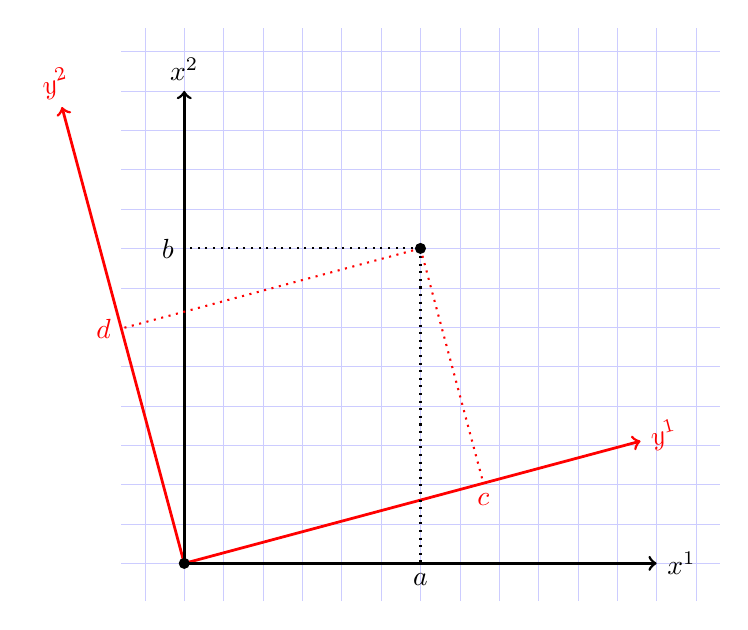
\begin{tikzpicture}[scale=2]
  \draw[step=.25cm,mjcgrid] (-0.4,-0.24) grid (3.4,3.4);
  \pgfsetlinewidth{1pt}

  \def\a{15}
  \coordinate (o)  at (0,0);
  \coordinate (ox) at (3,0);
  \coordinate (oy) at (0,3);
  \coordinate (p)  at (1.5,2);
  \coordinate (c)  at (canvas polar cs:angle=\a,radius=3cm);
  \coordinate (d)  at (canvas polar cs:angle=90+\a,radius=3cm);

  \draw [->,red] (o) -- (c); 
  \draw [->,red] (o) -- (d); 
  \draw [->]     (o) -- (ox); 
  \draw [->]     (o) -- (oy); 

  \pgfsetlinewidth{0.75pt}
  \draw [dotted] (p) -- ($(o)!(p)!(ox)$); 
  \draw [dotted] (p) -- ($(o)!(p)!(oy)$); 
  \draw [dotted,red] (p) -- ($(o)!(p)!(c)$);
  \draw [dotted,red] (p) -- ($(o)!(p)!(d)$);
  \pgfsetlinewidth{1pt}
  \node [below]  at ($(o)!(p)!(ox)$)  {$a$};
  \node [left]   at ($(o)!(p)!(oy)$)  {$b$};
  \node [below,red]  at ($(o)!(p)!(c)$)  {$c$};
  \node [left,red]   at ($(o)!(p)!(d)$)  {$d$};
  \node [right]  at (ox) {\textbf{$x^1$}};
  \node [above]  at (oy) {\textbf{$x^2$}};
  \node [rotate=\a,right,red] at (c) {\textbf{$y^1$}};
  \node [rotate=+\a,above,red] at (d) {\textbf{$y^2$}};
  \fill (p) circle (1pt);
  \fill (o) circle (1pt);
\end{tikzpicture}
\end{center}
\caption{\small The same point will have different coordinates when the basis vectors are different.}
\end{figure}


\begin{equation}
   d\phi = \sum_n \dd{\phi}{x^n} dx^n
\end{equation}

How does a change in gradient in the $x$ frame of reference relate to the change of gradient
in the $y$ frame of reference? In other words

$$
   \dd{\phi}{y^n} \quad ? \quad  \dd{\phi}{x^n}  
$$

we figure this out by using the chain rule of differentiation. For example for the $y^1$ component

$$
   \dd{\phi}{y^1}  = \dd{\phi}{x^1}\dd{x^1}{y^1} + \dd{\phi}{x^2}\dd{x^2}{y^1}  
$$
or in general

\begin{equation}
   \dd{\phi}{y^n} = \sum_m \dd{\phi}{x^m}\dd{x^m}{y^n}
\end{equation}

\subsection{Tensors}

Tensor of rank 0 is a scalar

Tensor of rank 1 is a vector

\begin{equation}
    V_y^n = \sum_m \dd{y^n}{x^m} V_x^m
\end{equation}

Tensor of rank 2 are relations between vectors

$$
   T^{mn} = A^m B^n
$$

$$
    A_y^m B_y^n = \sum_n \dd{y^m}{x^r} A_x^r  \sum_s \dd{y^n}{x^s} B_x^s 
$$

\begin{equation}
   T_y^{mn} = \sum_{r,s} \dd{y^m}{x^r} \dd{y^n}{x^s} T_x^{rs}
\end{equation}
This is called the contravariant transformation from x frame of reference to y frame of reference.

\begin{equation}
   T_{mn}(y) = \sum_{r,s} \dd{x^r}{y^m} \dd{x^s}{y^n} T_{rs}(x)
\end{equation}
This is called the covariant transformation from x frame of reference to y frame of reference.

\subsection{Metric tensor}

Insert triangle with side connotations

$$
   ds^2 = \sum_m dx^m dx^m
$$

$$
   ds^2 = \sum_{mn} dx^m dx^n \delta_{mn} =  \delta_{mn}\sum_{mn} dx^m dx^n
$$
now using 

$$
   dx^m = \sum_{r} \dd{x^m}{y^r} dy^r
$$
we get

$$
  ds^2 = \delta_{mn} \sum_{m,n,r,s} \dd{x^m}{y^r} dy^r \dd{x^n}{y^s} dy^s 
$$
or by rearranging,
$$
  ds^2 = \delta_{mn} \sum \dd{x^m}{y^r}  \dd{x^n}{y^s} dy^r dy^s 
$$
The term 
$$
   \delta_{mn} \sum \dd{x^m}{y^r}  \dd{x^n}{y^s}  
$$
is called the metric tensor, $g_{rs}$, and so we get

$$
  ds^2 = g_{rs} dy^r dy^s 
$$


\subsection{Christoffel symbols}

If two tensors are equal in one frame of reference (x) then they must 
be equal in any other frame of reference (y)

$$
   W_{mn}(x) = V_{mn}(x) \Rightarrow W_{mn}(y) = V_{mn}(y) 
$$

But this does not hold for derivatives. So if T is the derivative of V in frame $(x)$, 
$$
   T_{mn} (x) = \dd{V_m}{x^n} (x)
$$
then it is generally NOT true that 
$$
   T_{mn} (y) = \dd{V_m}{y^n} (y)
$$

Let us see why

$$
   T_{mn}(y) = \sum \dd{x^r}{y^m}\dd{x^s}{y^n} T_{rs}(x) =
     \sum \dd{x^r}{y^m}\dd{x^s}{y^n} \dd{V_r(x)}{x^s}
$$

$$
   T_{mn}(y) = \sum_r \dd{x^r}{y^m} \dd{V_r(x)}{y^n}
$$
now we have to check if

$$
   \sum_r \dd{x^r}{y^m} \dd{V_r(x)}{y^n} ?= \dd{V_m(y)}{y^n}
$$

using equation ()
$$
  \dd{V_m(y)}{y^n} = \dd{}{y^n} \left ( \sum_r \dd{x^r}{y^m} V_r(x)  \right )
$$
using differentiation of a product, we get

$$
   \dd{V_m(y)}{y^n} = \sum_r \dd{x^r}{y^m}\dd{V_r(x)}{y^n} + \frac{\partial^2x^r}{\partial y^n\partial y^m } V_r(x)
$$
or
$$
   \dd{V_m(y)}{y^n} = T_{mn}(y) + \sum_r \Gamma_{mn}^r V_r(x)
$$
or
$$
 T_{mn}(y) =  \dd{V_m(y)}{y^n} - \sum_r \Gamma_{mn}^r V_r(x)
$$

Covariant derivative.

$$
   \nabla_{y^n}V_m(y) = \dd{V_m(y)}{y^n} + \sum_r \Gamma_mn^r V_r(x)
$$


\end{document}
